%stpapb

\documentclass[../../main/main.tex]{subfiles}


\begin{document}
\title{STPA on Patrol Base Operations}

%%%%%%%%%%%%%%%% STPA on Patrol Base Operations %%%%%%%%%%%%%%%%
\chapter{STPA on Patrol Base Operations}\label{chp:stpapb}


%%%%%%%%%%%%%%%% Step 1 %%%%%%%%%%%%%%%%
\section{Step 1: Define The Purpose of The Analysis}\label{chp:stpapb:purpose}
\subsection{Organization FMA}

   %%%%%% table: organization goals %%%%%%%%%%
\begin{table}[h!]
\parskip=8pt
\begin{tabular}{||  m {7.5cm}  |  m {7.5cm}  ||}
\hline
\multicolumn{2} {|| c ||} {Organization Goals} \\
 \hline
U.S. Army Rangers	& U.S. Army\\
\hline
"The Rangers' primary mission is to engage the enemy in close combat and direct-fire battles. This mission includes direct action operations, raids, personnel and special equipment recovery, in addition to conventional or special light-infantry operations."
&	
The U.S. Army?s mission is to fight and win our Nation?s wars by providing prompt, sustained land dominance across the full range of military operations and spectrum of conflict in support of combatant commanders.\\
\hline
\end{tabular}
\caption{Organization goals.}
\label{orgo}
\end{table}
   %%%%%% table: organization goals %%%%%%%%%%
%%
\clearpage

\subsection{Patrol Base Operations FMA}
   %%%%%% table: PB FMAs  %%%%%%%%%%
\begin{table}[h!]
\parskip=8pt
\begin{tabular}{||  m {3cm}  |  m {12cm}  ||}
\hline
\multicolumn{2} {|| c ||} {Patrol Base Operations FMA} \\
 \hline
What &	establish a security perimeter when a squad or platoon halts for an extended period of time\\
\hline
How	&      planning, reconnaissance, security, control, and common sense\\
\hline
Why	&      avoid detection:
\begin{itemize}
\item hide a unit during a long, 
\item detailed reconnaissance; 
\item perform maintenance on weapons, 
\item equipment, eat, and rest; 
\item plan and issue orders; 
\item reorganize after infiltrating an enemy area; 
\item establish a common base from which to execute several consecutive or concurrent operations.
\end{itemize}\\
\hline
\end{tabular}
\caption{Patrol Base Operations Functional Mission Analysis.}
\label{pbfma}
\end{table}
   %%%%%% table: PB FMAs  %%%%%%%%%%
%%
\clearpage

\subsection{Assumptions about The System}
\begin{itemize}
\item Mission is decided by higher-ups and is provided as an input to the patrol base operations.
\item Mission is not changeable by the patrol base itself (exceptions are mission-specific).
\item Soldiers are deemed fit for duty before the mission commences.   (There may be exceptions.)
\item Soldiers are battle ready, but may not be fully mission capable (i.e., soldiers may require additional equipment and preparation that is mission-specific and determined after the mission is received).
\item The patrol base operations begin when the platoon (or patrol) leader receives order that there will be a mission.
\item The patrol base operations end when the patrol returns to the larger unit and has completed any debriefing required by the mission.
\item Other inputs to the system are intelligence from the larger unit (higher-up HQ), intelligence from other units (if applicable), and intelligence gathered during the mission from the mission itself. 
\item Feedback is received from the platoon regarding carrying out orders and from the operations themselves regarding completion of tasks, etc.  
\item Adversary also may input information to the platoon leader (by interfering with communications from higher-up HQ), to the platoon soldiers (by interfering with intra-patrol communications), and to the operations themselves (by disrupting on the operations in various forms, including contact).
\end{itemize}


\subsection{System Entities}
\begin{itemize}
\item PL, PSG, 
\item Medic, FO, RTO, HWSQL
\item Squad Leaders
\item Fire Team Leaders
\item Buddy Team
\item Soldiers
\item Adversary (enemy)
\end{itemize}

%%
\clearpage
\subsection{Accidents/Losses}
   %%%%%% table: Accidents/Losses  %%%%%%%%%%
\begin{table}[h!]
\parskip=8pt
\begin{tabular}{||  m {2cm}  |  m {13cm}  ||}
\hline
\multicolumn{2} {|| c ||} {Accidents/Losses} \\
\hline
	&Description\\
\hline
L1	&MIA, KIA, WIA, CIA\\
\hline
L2	&Wrong mission\\
\hline
L3	&Mission Failure\\
\hline
L4	&Negative publicity/exposure/unwanted attention\\
\hline
L5	&Equipment loss/damage/capture by enemy\\
\hline
L6	&Civilian casualties/disruption to local population\\
\hline
L7	&Insufficient communications with high-up HQ\\
\hline
\end{tabular}
\caption{System accidents/losses.}
\label{losses}
\end{table}
   %%%%%% table: Accidents/Losses  %%%%%%%%%%

%%
\clearpage
\subsection{System-level Hazards/Vulnerabilities And Constraints}
  %%%%%% table: System-level hazards  %%%%%%%%%%
\begin{table}[h!]
\parskip=8pt
\begin{tabular}{|  m {0.7cm}  |  m {4.5cm} |  m{3.5cm}   |   m {0.7cm} |  m {4.5cm}   |}
\hline
\multicolumn{5}{| c |}{Hazards/Vulnerabilities and constraints}\\
\hline
\multicolumn{2}{| c |}{System-level Hazards/Vulnerabilities} & \multicolumn{1}{| c |}{Accidents/Losses} & \multicolumn{2}{| c |}{System-level Constraints}\\
\hline
H1    &Insufficient planning		&L1, L2, L3, L4, L5, L6, L7	&SC1	&Plan sufficiently\\
\hline
H2	&Insufficient reconnaissance/intelligence	&L1, L2, L3, L4, L5, L6, L7	&SC2	&Reconnoiter sufficiently\\
\hline
H3	&Insufficient security			&L1 ,L3, L4, L5, L6		&SC3	&Provide sufficient security\\
\hline
H4	&Insufficient control			&L1, L2, L3, L4, L5, L6 ,L7	&SC4	&Maintain adequate control\\
\hline
H5	&Insufficient common sense	&L1, L2, L3, L4, L5, L6, L7	&SC5	&Use common sense\\
\hline
H6	&Insufficient leadership		&L1, L2, L3, L4, L5, L6, L7	&SC6	&Establish sufficient leadership\\
\hline
H7	&Insufficient communication with higher-HQ	&L1, L2, L3, L4, L5, L6, L7	&SC7	&Maintain sufficient communications with higher-HQ\\
\hline
H8	&Insufficient haste			&L1, L3	&SC8	&Maintain appropriate pace\\
\hline
H9	&Disregard for Rules of Engagement  &L4, L6	&SC9	&Follow Rules of Engagement\\ 
\hline
\end{tabular}
\caption{System-level hazards/vulnerabilities and constraints.}
\label{hazards}
\end{table}
  %%%%%% table: System-level hazards  %%%%%%%%%%
%%
\clearpage
%%%%%%%%%%%%%%%% Step 2 %%%%%%%%%%%%%%%%
\section{Step 2: Model The Control Structure}\label{chp:stpapb:control}
\subsection{Controllers And Process Models}
 %%%%%% table: Controllers Processes %%%%%%%%%%
\begin{table}[h!]
\parskip=8pt
\begin{tabular}{|  m {3cm}  |  m {3cm}  |  m {3cm}     |  m {5cm}   |}
\hline
\multicolumn{4}{| c |}{Controllers And Process Model}\\
\hline
Controller & Model & Variables & Values\\
\hline
\multirow{2}{3cm}{Platoon Leader}	& Patrol Base \newline Status	& State	 &
\begin{itemize}
\item PLAN_PB
\item MOVE_TO_ORP
\item CONDUCT_ORP
\item MOVE_TO_PB
\item CONDUCT_PB
\item COMPLETE_PB
\item ABORT_PB
\end{itemize}\\
\cline{2-4}
      & Policy  & Authenticated &
 \begin{itemize}
\item True
\item False
\end{itemize}\\
\hline
Platoon	& Authentication Model	& Authenticated	 &
\begin{itemize}
\item True
\item False
\end{itemize}\\
\hline
Adversary	& Threat Model	& To be \newline determined & to be determined\\
\hline
\end{tabular}
\caption{Controllers and process model.}
\label{controlprocess}
\end{table}
 %%%%%% table: Controllers Processes %%%%%%%%%%
 %%
\clearpage

\subsection{Control Actions}
The control actions for each principal are listed below.
\begin{itemize}
\item Platoon Leader
\begin{itemize}
\item PL says crossLD (same as planComplete)
\item PL says conductORP
\item PL says moveToPB
\item PL says completePB
\item PL says reactToContact
\item PL says returnToBase
\item PL says changeMission
\end{itemize}
\item Platoon
\begin{itemize}
\item exec(crossLD) (same as planComplete)
\item exec(conductORP)
\item exec(moveToPB)
\item exec(completePB)
\item exec(reactToContact)
\item exec(returnToBase)
\item exec(changeMission)
\end{itemize}

\end{itemize}

\subsection{Functional Control Structure}
%%
\clearpage

\begin{figure}[ht!]
\begin{center}
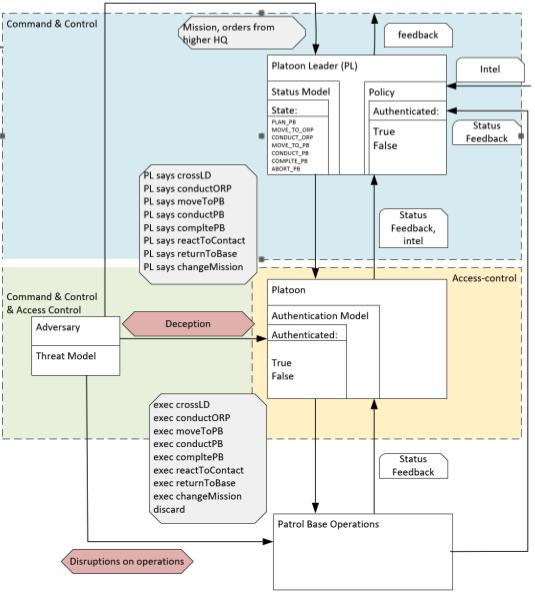
\includegraphics[width=0.7\linewidth]{../figures/controlstr1}
\caption{Control structure for patrol base operations.}
\label{controlstr1}
\end{center}
\end{figure}

%%
\clearpage

%%%%%%%%%%%%%%%% Step 3 %%%%%%%%%%%%%%%%
\section{Step 3: Identify Unsafe Control Actions (UCAs)}\label{chp:stpapb:uca}
The Thomas methods is used to identify \glspl{uca}.

\subsection{Unsafe Control Actions (UCAs): Thomas Model}
%%
\clearpage
\paragraph*{PL says planComplete}
The Thomas method for delineating \glspl{uca} for \textit{PL says planComplete} are shown in figure \ref{UCAPLsays}.
\begin{figure}[ht!]
\begin{center}
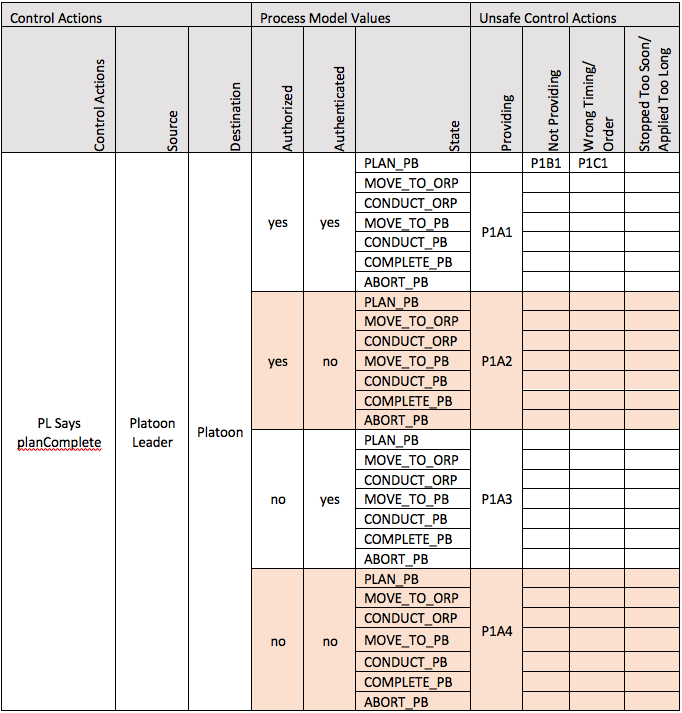
\includegraphics[width=\linewidth]{../figures/UCAPLsays}
\caption{Unsafe control actions \glspl{uca} for control action "PL says planComplete."}
\label{UCAPLsays}
\end{center}
\end{figure}

%%
\clearpage
\paragraph*{exec(planComplete)}
The Thomas method for delineating \glspl{uca} for \textit{exec(planComplete)} are shown in figure \ref{UCAPLsays}.
\begin{figure}[ht!]
\begin{center}
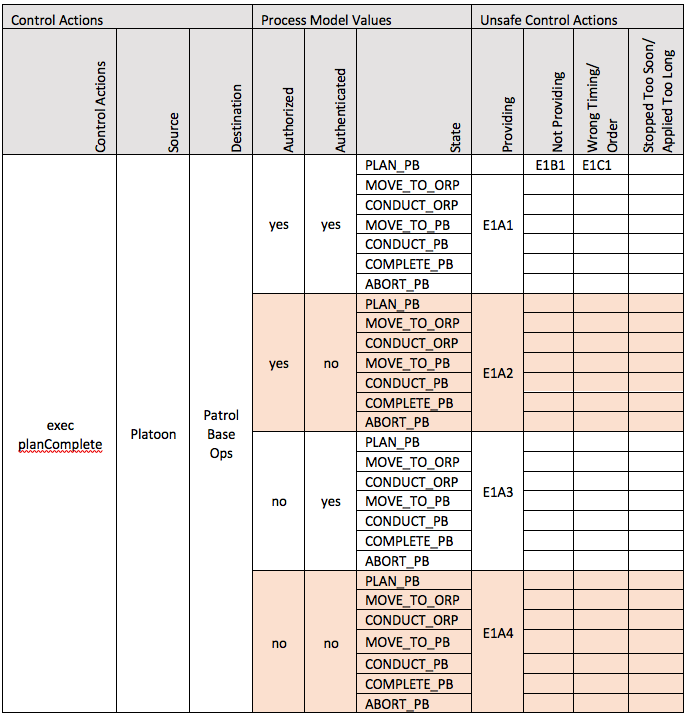
\includegraphics[width=\linewidth]{../figures/UCAexecplan}
\caption{Unsafe control actions \glspl{uca} for control action "exec(planComplete)."}
\label{UCAexecplan}
\end{center}
\end{figure}

%%
\clearpage
\paragraph*{discard(anyCommand)}
The Thomas method for delineating \glspl{uca} for \textit{discard{anyCommand}} are shown in figure \ref{UCAPLsays}.
\begin{figure}[ht!]
\begin{center}
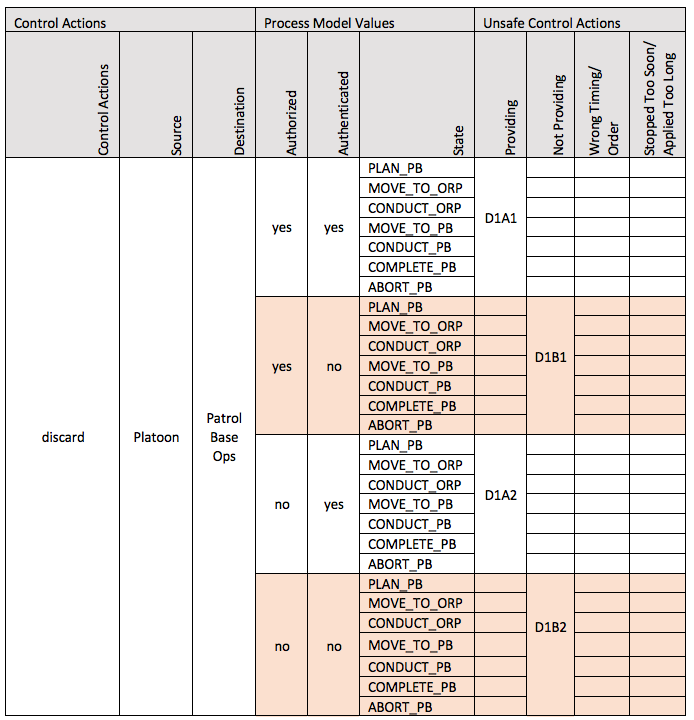
\includegraphics[width=\linewidth]{../figures/ucadiscards}
\caption{Unsafe control actions \glspl{uca} for control action "discard(anyCommand)."}
\label{UCAdiscard}
\end{center}
\end{figure}
%%
\clearpage
%%%%%%%%%%%%%%%% Step 4 %%%%%%%%%%%%%%%%
\section{Step 4: Identify Loss Scenarios}\label{chp:stpapb:scenarios}
\subsection{Scenarios}

\subsubsection*{Pl says planComplete}
%%
\clearpage
\paragraph*{P1B1/P1C1: state = PLAN_PB, Authorized = Yes, Authenticated = Yes}

\begin{figure}[ht!]
\begin{center}
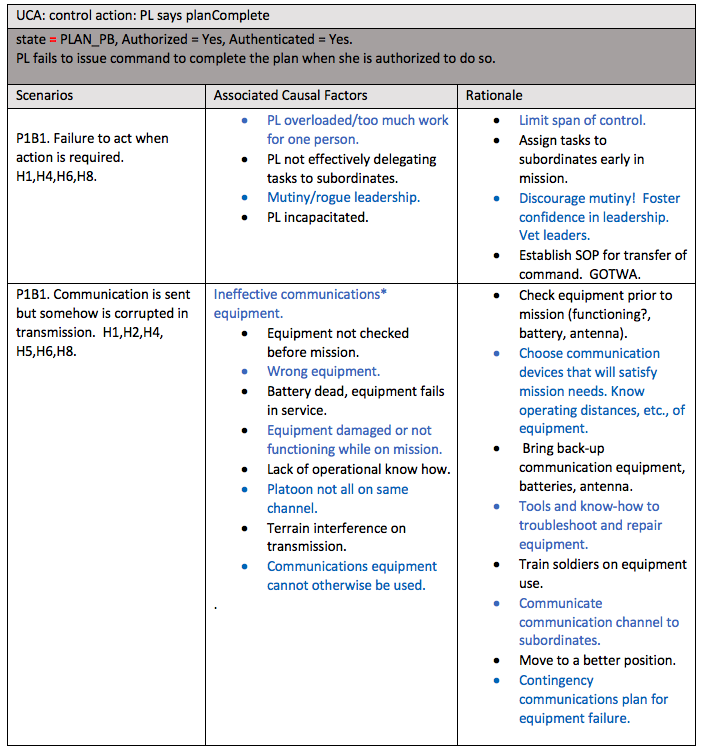
\includegraphics[width=\linewidth]{../figures/ucap1b1}
\caption{Scenarios for UCA P1B1.}
\label{ucap1b1}
\end{center}
\end{figure}
%%
\clearpage


\begin{figure}[ht!]
\begin{center}
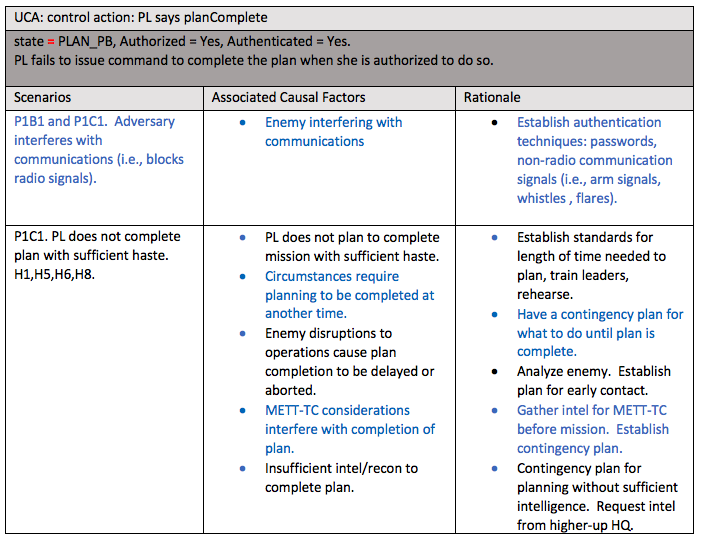
\includegraphics[width=\linewidth]{../figures/ucap1b1p1c1}
\caption{Scenarios for UCA P1B1/P1C1.}
\label{ucap1b1p1c1}
\end{center}
\end{figure}
%%
\clearpage



\paragraph*{P1A1: state  = PLAN_PB, Authorized = Yes, Authenticated = Yes}


\begin{figure}[ht!]
\begin{center}
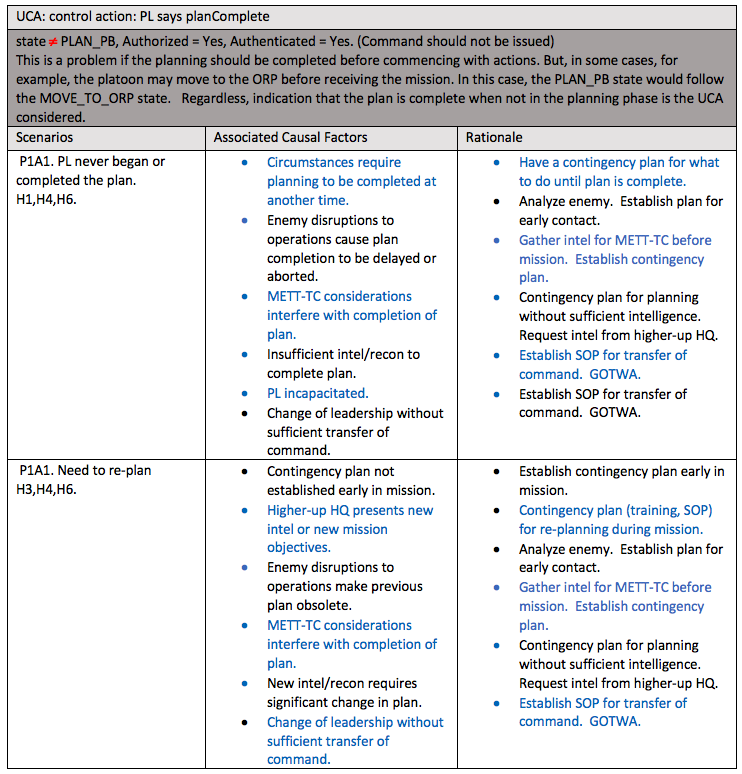
\includegraphics[width=\linewidth]{../figures/ucap1a1}
\caption{Scenarios for UCA P1A1.}
\label{ucap1a1}
\end{center}
\end{figure}
%%
\clearpage
\paragraph*{P1A2: state  = any state, Authorized = Yes, Authenticated = No}

\begin{figure}[ht!]
\begin{center}
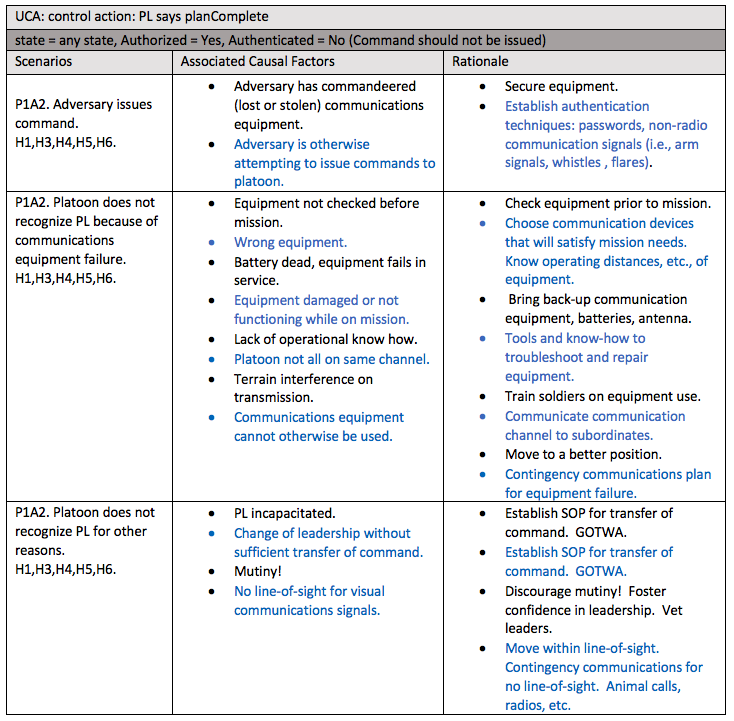
\includegraphics[width=\linewidth]{../figures/ucap1a2}
\caption{Scenarios for UCA P1A2.}
\label{ucap1a2}
\end{center}
\end{figure}

%%
\clearpage
\paragraph*{P1A3: state  = any state, Authorized = No, Authenticated = Yes}

\begin{figure}[ht!]
\begin{center}
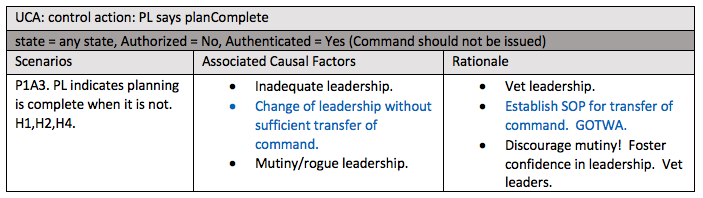
\includegraphics[width=\linewidth]{../figures/ucap1a3}
\caption{Scenarios for UCA P1A3.}
\label{ucap1a3}
\end{center}
\end{figure}

%%
\clearpage


\paragraph*{P1A4: state  = any state, Authorized = No, Authenticated = No}

\begin{figure}[ht!]
\begin{center}
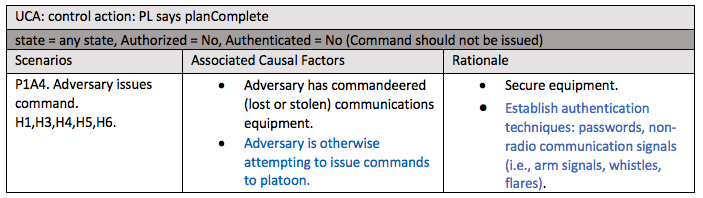
\includegraphics[width=\linewidth]{../figures/ucap1a4}
\caption{Scenarios for UCA P1A4.}
\label{ucap1a4}
\end{center}
\end{figure}
%%
\clearpage


\subsubsection*{exec(planComplete)}
\paragraph*{E1B1/E1C1: state = PLAN_PB, Authorized = Yes, Authenticated = Yes}

\begin{figure}[ht!]
\begin{center}
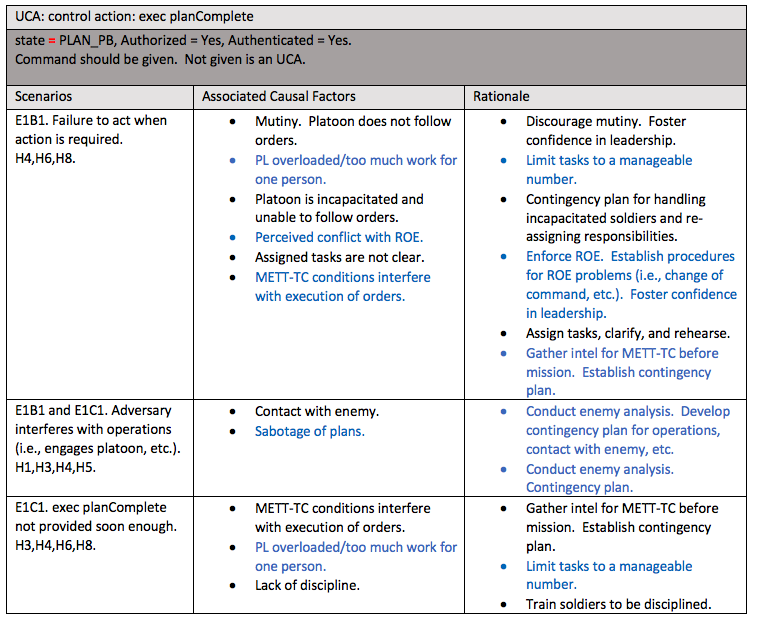
\includegraphics[width=\linewidth]{../figures/ucae1b1e1c1}
\caption{Scenarios for UCAs E1B1 and E1C1.}
\label{ucae1b1e1c1}
\end{center}
\end{figure}
%%
\clearpage

\paragraph*{E1A1: state  $\neq$ PLAN_PB, Authorized = Yes, Authenticated = Yes}

\begin{figure}[ht!]
\begin{center}
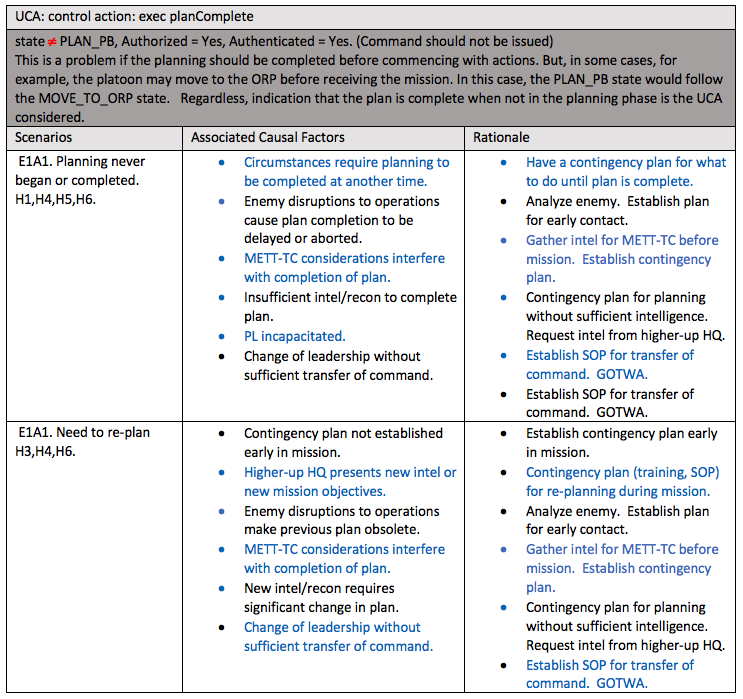
\includegraphics[width=\linewidth]{../figures/ucaea1}
\caption{Scenarios for UCA E1A1.}
\label{ucaea1}
\end{center}
\end{figure}
%%
\clearpage
\paragraph*{E1A2: state  = any state, Authorized = Yes, Authenticated = No}
\begin{figure}[ht!]
\begin{center}
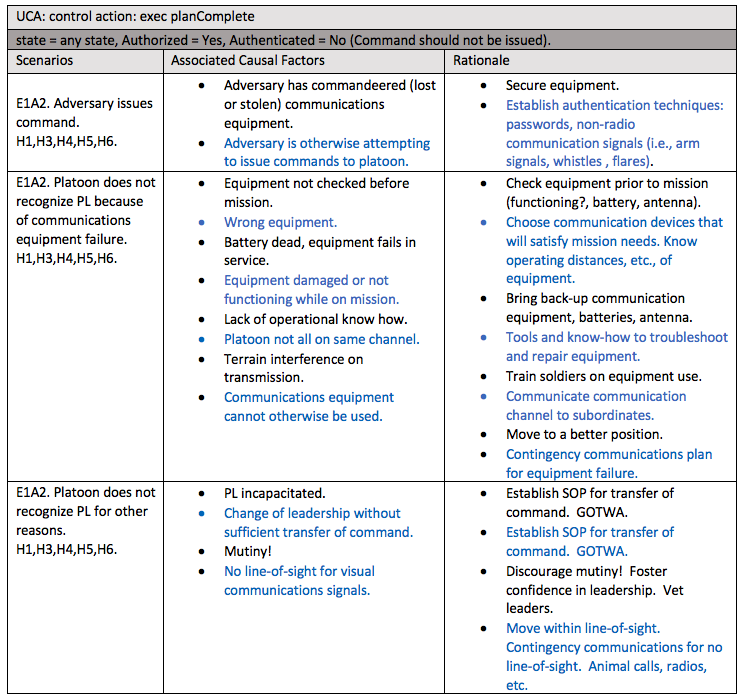
\includegraphics[width=\linewidth]{../figures/ucae1a2}
\caption{Scenarios for UCA E1A2.}
\label{ucae1a2}
\end{center}
\end{figure}
%%
\clearpage

\paragraph*{E1A3: state  = any state, Authorized = No, Authenticated = Yes}

\begin{figure}[ht!]
\begin{center}
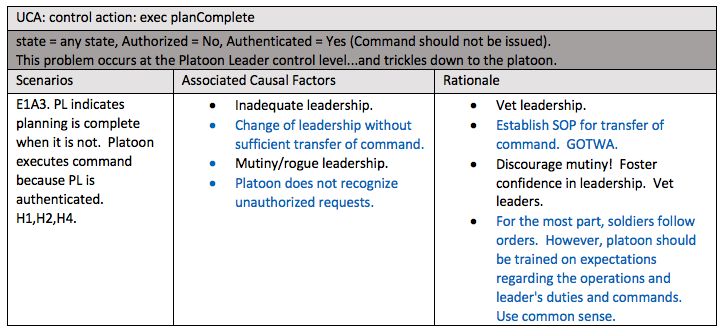
\includegraphics[width=\linewidth]{../figures/ucae1a3}
\caption{Scenarios for UCA E1A3.}
\label{ucae1a3}
\end{center}
\end{figure}
%%
\clearpage


\paragraph*{E1A4: state  = any state, Authorized = No, Authenticated = No}

\begin{figure}[ht!]
\begin{center}
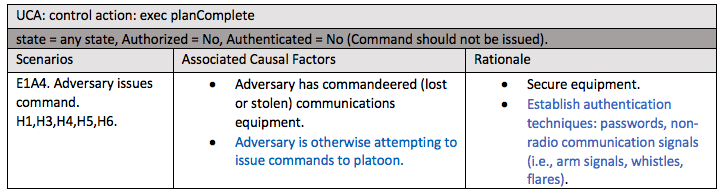
\includegraphics[width=\linewidth]{../figures/ucae1a4}
\caption{Scenarios for UCA E1A3.}
\label{ucae1a4}
\end{center}
\end{figure}
%%
\clearpage


\subsubsection*{discard(anyCommand)}

\begin{figure}[ht!]
\begin{center}
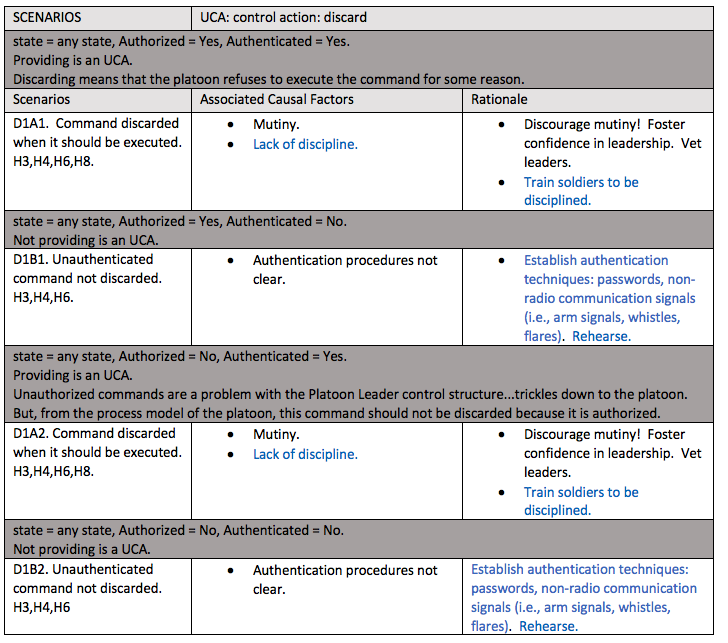
\includegraphics[width=\linewidth]{../figures/ucadiscard}
\caption{Scenarios for UCA for discard on all commands (D1A1 through D1A4).}
\label{ucadiscard}
\end{center}
\end{figure}
%%
\clearpage

%%%%%%%%%%%%%%%% Discussion %%%%%%%%%%%%%%%%
\section{Discussion And Conclusions}\label{chp:stpapb:discuss}


\end{document}